\chapter{Understanding The Behaviour of Retweeting in Twitter}


Stuff to finish up in this section:
\begin{itemize}
\item Explain motivation for research in this particular area
\item Use this motivation to explain the purpose for this research as a basis for the work in the next few chapters
\item Explain how this chapter is the basis for research into Twitter's social structure in the next chapter
\item Normalise terms (retweet-group size / retweet volume) here and in further chapters throughout thesis
\item (thinking forward: e.g. we have addressed tweet quality in terms of propagation, can a network have a quality too? what further factors can affect the dissemination of information in social networks?
\end{itemize}

It has been discussed that the popularity of information in Twitter can be related to the propagation characteristics of that information through Twitter's social structure. That is to say, that the more times a Tweet is retweeted by users, the more people have found the information contained within it to be interesting enough to be worth sharing.\\
It has also been shown that this retweet count metric alone cannot be an implication of the actual interestingness level of a Tweet. This is related to the notion of user influence, which directs that some tweets are naturally immediately seen by more people and thus have a higher chance of achieving a retweet as they are. Indeed, since follower count is one of the \cite{suh10} demonstrated that a user's Tweets' retweet rates increase as the user's follower count increases.

The strength of Twitter lies is in its social structure, where users can elect to follow and unfollow others as they choose. Followers of a user receive all of that user's posts in their individual (or `home') timelines. If a user has set their profile to be public, then their posts also used to appear on the public timeline, which is now deprecated but was accessible to anyone; even those without a Twitter account. As a result, people are likely to follow users who update with interesting posts; whether the follower is a big fan of the user and simply wants to know everything going on in their life, or if the follower is simply interested in the topical area of most of the friend's posts. 

Just as Twitter users will post Tweet about topics that are of interest them - possibly related to a user's work, a hobby, or a mixture of multiple areas - and these Tweets are generally posted with the idea that they will be useful or interesting for some of their followers as well as an attempt to attract more followers, retweets are generated with the same motives in mind. This means that if a Tweet is retweeted, it is not only allowed to disseminate further through the social structure, but also that a higher Tweet quality is implied.

Thus, this describes how a user's friends, who carry out retweets, effectively become filters of interesting information for that user and other followers of those friends, and the \textit{audience} of the original Tweet is significantly increased. Since retweets are always attributed to the original author then you, a Twitter user, may gain more attention by means of followers by posting \textit{interesting} Tweets, which will; 
\begin{enumerate}
\item increase the chances that users reading your Tweets will choose to follow you, and
\item increase the chances that users will decide to retweet your Tweet, thus broadcasting it to a larger audience. People viewing this \textit{retweet} then may decide to follow you. 
\end{enumerate}

Since a Tweet can be retweeted multiple times, and, as mentioned, a retweet itself can also be retweeted, the much larger the effective audience (both directly and through retweets) of a Tweet's original author has the potential to become if they choose to post interesting information. In this chapter, an understanding of the behaviours and properties of retweets is provided, along with discussions into how these are relevant in determining useful metrics for determining which retweeted information is interesting.


\section{Tweet and Retweet Properties}

\subsection{Retweet Groups}
A Tweet has various attributes associated with it, which make up the features that describe that particular Tweet. Each Tweet has a set of properties relating to its content, its author, and other metadata, such as creation time.\\
As such, a particular Tweet, $t$, can have its relevant properties declared and be defined as follows;
\[
	t = (\mathrm{text}, \mathrm{count}_R, \mathrm{author}_O, \mathrm{author}_R, \mathrm{orig})
\]

Respectively, this represents the Tweet's text, its retweet count, and the \textit{original} author of the Tweet. The final two values depend on whether $t$ is a retweet or not and represent the author of the retweet and the original Tweet respectively. Since a retweet remains a class of Tweet, then the same properties can be assigned to retweets as to Tweets, except that in the case of retweets the values $\mathrm{orig}$ and $\mathrm{author}_R$ will be non-null.

Since a Tweet can be retweeted more than once, the set of Tweets that are in the set of \textit{all} Tweets, $T$, and are retweets of $t$ is defined as;
\[
	RT(t) = \left\{ s \in T : s.\textrm{orig} = t \right\}
\]

Clearly, the retweet count of $t$, $ t.\mathrm{count}_R = \left\vert{RT(t)}\right\vert $.

An original Tweet, $t$, along with all of the retweets of $t$, $RT(t)$, are known as the \textit{retweet group} of $t$, which is defined as $G(t)$ and is useful when discussing the audience reach of a particular Tweet. Therefore, since $t$ is also a member of this set, the size of $t$'s retweet group is; 
\[
	\left\vert{G(t)}\right\vert = t.\mathrm{count}_R + 1 
\] 
If $ r_1,...,r_n $ are the members of $RT(t)$ then the raw audience size of the group can be calculated thus (assuming $t.\textrm{count}_R \geq 1$);
\[
	\textrm{audience}(G(t)) = \textrm{followers}(t.\textrm{author}_O) + \sum\limits_{i=1}^{t.\mathrm{count}_R} \textrm{followers}(r_i.\textrm{author}_O)
\]

However, properties of Twitter dictate that this raw audience size is not an accurate calculation in most cases, as is discussed later in this chapter.


\subsection{Retweet Trees}
As a Tweet gains in popularity and attracts more and more retweets to be created from it, and since retweets themselves can also be retweeted, then this ultimately results in the generation of a retweet \textit{tree}, which represents the retweet group of a particular Tweet. This tree is formed from the \textit{users} who have retweeted the Tweet (or a retweet of the Tweet), and represents the original Tweeter and the various pathways taken by the Tweet as it is retweeted through the social graph.

The tree is not a representation of the actual social ties between the tree's nodes, as users are able to retweet Tweets and retweets sent from others that they do not follow. However, as is mentioned later in this chapter, most retweeting does generally occur between directly-linked users.

The root of the tree representing every $G(t)$ is $t.\textrm{author}_O$ and, if $t$ has been retweeted, each of the other nodes are $$r_1.\textrm{author}_R, ... , r_n.\textrm{author}_R \: \forall \: 1 \leq n \leq t.\mathrm{count}_R $$\\
A similar illustrative device is used by \cite{galuba10} in describing URL \textit{cascades} in Twitter.

\begin{figure}[h]
\centering
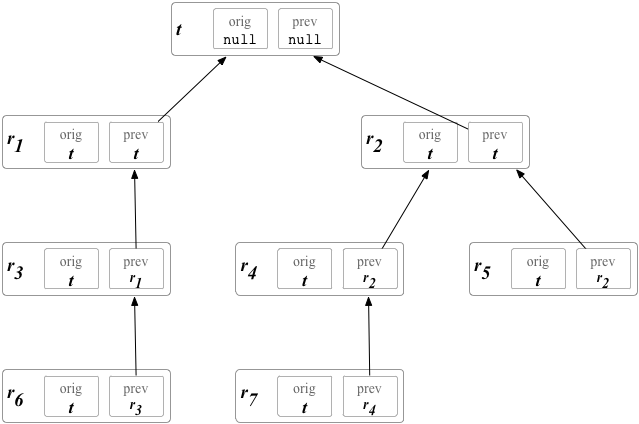
\includegraphics[scale=0.5]{3.Chapter1/Media/tree.png} 
\caption{\textit{A hypothetical retweet pathway tree.}}
\label{fig:retweet_tree}
\end{figure}

Although these retweet pathways can technically be acyclic through the use of the manual retweet method, the case of a user retweeting a Tweet more than once is very rare and a user retweeting a retweet that they are already part of the upstream chain of is even less likely to occur. The retweet button method simply does not support users retweeting a Tweet more than once.\\
As such, retweet trees are used in preference over retweet \textit{graphs} as they illustrate the temporal nature in terms of the order in which the retweets occur.


\subsection{Path-Length}
In addition to retweet groups having a size property, a retweet groups's branch's \textit{path-length} refers to the length of a particular retweet chain. In particular, it defines the number of times a Tweet is retweeted down one chain from the source user (the retweet group's tree's root) down to the final retweeter in the chain (a tree's leaf node).

Figure \ref{fig:retweet_tree} represents the users in the retweet group of a hypothetical Tweet.\\
This retweet group has a size of 11 and has 7 distinct retweet chains, the longest of which is the one traversing users 1, 3, 6 and 11.\\
The \textit{maximum} path-length of this retweet group is therefore 3, as the leaf node of this branch is three hops away from the original author at the root.

As has been mentioned previously, when a user retweets a Tweet or retweet through the manual approach, it involves pre-pending the current state of the Tweet with the text \texttt{RT @<username>:}.\\
Therefore, the Tweet with the content;\newline
\texttt{RT @user2: RT @user1: This is the body of the Tweet}\newline
was originally authored by \texttt{user1}, then retweeted by \texttt{user2}, and then finally retweeted by the author of this current retweet (the author of a Tweet or retweet's username is not credited in the body of the text).

It should be noted that this phenomenon can only be observed through retweets by the manual approach, since the button method always simply credits the original author, and not any of the internal members of the retweet group.

Although most retweets today are carried out using the button method, the manual approach still remained popular at the time the research in this chapter was carried out. This allowed for making useful observations of retweet patterns that would not be as prevalent later on.


\section{More on Information Retrieval}
A Twitter user electing to follow another user cannot predict precisely what the new friend will Tweet about in the future. The user has some \textit{expectation} of the type of information they are likely to receive based on the previous Tweets of the new friend, which is generally the only cue the user can use to base the follow decision on.

Part of the follow decision is based on the notion of relevance judgement, which is a notion discussed at more length by \cite{xu07} and is partly made up of the goal of achieving \textit{affective stimulation} through \textit{hedonic} searching as opposed to the use of \textit{epistemic} searching.

\subsection{Epistemic Search}
An epistemic information search is one that involves carrying out a search with the purpose of finding out information on a particular topic (or set of) to satisfy a \textit{desire for knowledge} \cite{xu10}, yet without an actual aim to solve any particular problem.

An example of this type of search is a `crawl' through Wikipedia, in which a searcher may start at one particular page of interest and then follow links within that page to other related pages of interest that stem away from the source topic. In this case, the search `parameter' is simply the name or title of the article the searcher wants to view.\\
As mentioned previously, a followship between users is effectively a search parameter in Twitter, since the following user has elected to follow the new friend to receive information from him/her. It is clear that this type of `searching' cannot be epistemic as the following user cannot know exactly the type of information they are going to receive.

\subsection{Hedonic Search and Affective Stimulation}
Hedonic searching is similar to epistemic searching in that it is also not carried out with the aim to solve an immediate problem, but is different in that it is done to search for fun or `affective stimulation' \cite{xu10}.

A person can be said to be affectively stimulated if they view a piece of information that has some effect on the person, such as an emotional effect, something that is of particular interest to the person, or something that is capable of provoking some further thought.

With hedonic searching, users are not aware of the information that they are going to receive prior to searching and thus cannot really predict any level of affective stimulation.\\
This aligns more with Twitter usage, since users receive information that they cannot accurately predict. Any Tweets received that do and provide interesting information convey affective stimulation to the user. This is the type of information that becomes harder to identify amongst lots of noise, yet is also the type of information a user is more likely to retweet.

\subsection{The Recognition Heuristic} 
A further metric for measuring information relevance in information retrieval is the recognition heuristic.\\
The recognition heuristic takes advantage of a person's memory and declares that if a person is able to recognise only one of two (or more) items, then he/she is more likely to judge the recosnided item to be `greater' or more important \cite{oppenheimer03} \cite{goldstein99}.

Relating this to information received on Twitter, \cite{chorley12} found that a user recognising a Tweet's author significantly increases the chance that the user will decide to read the Tweet. Since a user must read a Tweet in order to make a decision on whether, or not, to retweet it, then the recognition heuristic transiently plays a part in a user's retweet decision also.

The authors also find that information about the Tweet itself, such as its text content and its retweet count, has much more of an effect on a user's read decision than information about the author, such as the followers count or Tweet rate. This also contributes to the declaration that information interest goes beyond the features surrounding a particular user and that user influence does not dictate interestingness of information.


\section{Twitter Analysis}


Discuss wanting to know more about Twitter and the way information is propagated through this. \\
Want to gain a base knowledge of some of the propagation patterns in terms of the tweets and the networks the tweets travel through. \\
This will form basis of research further on. \\ 
Stuff interested in:
\begin{itemize}
\item retweet groups (define)
\item path-length (define)
\item friend/follower graph 
\item timings, etc.
\end{itemize}

\section{Experimental Methods}
\label{experimental methods}
% take some of this and add to Twitter Analysis section (maybe will be renamed)
\subsection{Data Collection Methodology}
The experiments conducted involve the examination of tweets selected randomly from the Twitter public timeline\footnote{Viewable from \textit{http://www.twitter.com/} when not logged in.}. The system interfaces with the Twitter REST API and periodically retrieves the top 20 tweets from the timeline, filtering out the posts that are retweets. They are distinguishable as they start with the characters `RT' followed by a username. These retweets are then stored and the original tweet text is extracted. Sometimes retweets are made with additional text as comments, which made it harder to retrieve the actual original text. In these cases, additional queries are made to try and source the original text, but, failing that, the retweet is discarded.\\
The original text is then used to query all available tweets for the original tweet and any other retweets. The original tweet, along with its set of retweets is referred to as the \textit{retweet group}. As a result, each retweet group contains precisely one original tweet and at least one associated retweet, thus the smallest possible retweet group is of size two. The \textit{final retweeter} is the most recent person to retweet the post. Results are generated by extracting data from these retweet groups, which are stored with metadata such as time, source, language, and so on.\\
It should be noted that there are two ways in which tweets can be retweeted. The traditional (or \textit{old}) manner involved users copying the existing tweet (or retweet) from the timeline before tweeting that with the characters `RT' and the previous retweeters username at the start. This ensures that the appropriate users are cited as being the author of the tweet. The \textit{new} method enables users to retweet a post simply by clicking the `Retweet' button that is available next to the post on the timeline both on the main Twitter website and on various Twitter clients. Despite the fact that the website and clients have alternate ways of displaying these types of retweets, the search interfaces and API still see them as starting with `RT' and the previous poster's username. This, fortunately, means that both types of retweets can be collected in the same way. Retweeting in the latter method, however, is unavailable if the post that is to be retweeted belongs to a user who has a non-public profile.\\
Despite this, the new method doesn't have direct support for retweet chains (explained below) to be formed. No matter who retweeted the post previously (whether they were the original poster, or not), the new retweeting method simply treats it as a direct retweet from the original poster (as long as the previous retweets were also made in this fashion). The original tweet (and other retweets) can still be found using the search method outlined above, however, so this doesn't significantly affect results. Limitations with both the Twitter API and the search interfaces did mean that not all retweets could have successful queries made against them.\\
As briefly described above, these experiments use the notion that retweets themselves can be retweeted; analogous to routers forwarding packets in a multi-hop networking system.\\


\subsection{Data}
There are three sets of experiments detailed in the following section and all of the data was collected using the search method outlined above. The data consists of around 4400 retweet groups (representing a total of about 26,000 tweets and retweets) collected between 26th January \& 24th May 2011. It is acknowledged that this is a relatively small result set and so we emphasise that these are \textit{preliminary} experiments to provide insight into the decentralised side of Twitter and to act as a start point for future work in this area.\\

\section{Empirical Results}

\subsection{Length of Retweet Chains}
\label{length of retweet chains}
The longest path-length encountered from the dataset of retweet groups was 9, meaning that the tweet has been forwarded nine times from the original user; making the total number of involved users ten. Despite this, in the dataset, the average path-length was around 1.8, with the vast majority of tweets being retweeted between one and two times, as shown by the distribution in Figure \ref{fig:pathlength-distribution}. The \textit{maximum path-length} of a retweet group refers to the longest path-length present in the group.\\
\begin{figure}[h]
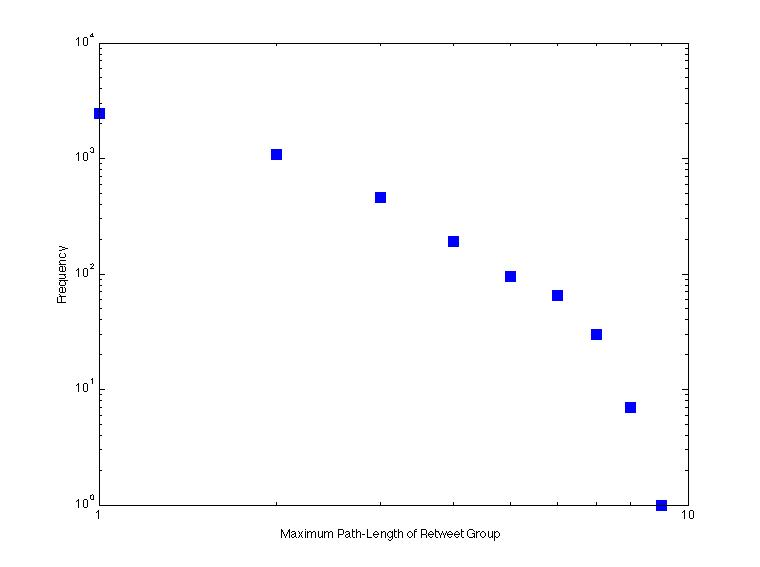
\includegraphics[scale=0.35]{3.Chapter1/Media/pathlength-distribution.jpg} 
\caption{\textit{Log/log distribution of maximum path-lengths from retweet groups.}}
\label{fig:pathlength-distribution}
\end{figure}
It should be noted that the very high proportion of single-chain path-lengths could be a result of the new method of retweeting introduced in the previous section, since, as mentioned, if all of the users in a retweet chain were to retweet in this way then Twitter would still only treat the path-length as one; between the original tweeter and each of the intermediate retweeters. Despite this, the result fits the rest of the dataset well.\\
This data can also be used to have a look at the friend-follower graph associated with retweets. In cases where the group's maximum path-length is equal to one (i.e. simply the case where a user has retweeted another user's tweet once), the retweeter follows the original tweeter about 90\% of the time. This implies that in 10\% of cases, a retweeting user has retweeted a tweet found outside of their home timeline, i.e. on the public timeline, or whilst browsing through other users. It could also be as a result of the retweeter not including the tweet citation (`@username') for reasons such as to save space, which would be particularly likely in cases of longer tweets. This implies that the more followers a user has, the greater chance that user has of having his or her tweets seen and of being retweeted. Since 90\% of retweets occur if the retweeting user follows the original tweeter, then this is directly demonstrated. However, this does not take into account whether the tweet was passed down a chain of retweets retweeted with the second (single click) method. In these cases the path-length would be represented with a length of one even if they were actually longer. The introduction of the second method of retweeting is, therefore, not helpful with the analysis of retweets.\\
In addition to this, in cases where the maximum path-length is greater than one (i.e. at least one user retweeting in a chain between original tweeter and final retweeter), the final retweeter follows the original tweeter in about 40\% of cases. From Figure \ref{fig:totalretweets-pathlength} we can see that retweet groups with a larger maximum path-length tend to be larger themselves. This means that the tweet has travelled further both around the original tweeter, but also potentially to other communities. Users from other communities will be less likely to follow this original tweeter, explaining this drop in likelihood. Results have also hinted that the probability of users citing the original tweeter decreases as the path-length of the retweet increases, which also goes some way to explain this point. 

\subsection{Size of Retweet Groups}
\label{size of retweet groups}
This section focuses on properties of retweet group size, and also how this can be related to path-length. The average retweet group size found from the data was of size 6, with the largest and smallest retweet groups being of size 284 and 2 respectively.\\

The distribution of retweet group sizes can be seen in Figure \ref{fig:retweet-distribution} and shows that this data follows a power-law distribution (with a relatively large \textit{p}-value of 0.871). The $Pr(X \geq x)$ represents the complementary cumulative distribution function, where the randomly generated \textit{X} is greater than or equal to \textit{x}. These values were calculated using the techniques and code provided by \cite{clauset07}.\\
In these retweet groups, and particularly the larger ones, retweets are likely to be down several chains. Combining this information with that of the average path-length of retweets, it becomes more clear how the retweet tree structure is created, with nodes being the retweeting users (the root node being the original tweeter), and edges between nodes being the path of retweets. Different retweet chains would be illustrated by the combinations of journeys down different branches. The longest path-length would be represented by the depth of the longest tree branch, and the total number of retweets would be represented by the number of edges. The trees can be said to represent the retweet groups, though, in practice, many members of the group will be separate from the main tree due to missing citations.\\
\cite{kwak10} discusses retweet trees in more detail, in particular, the different shapes of the trees representing retweet groups from the Air France incident. Their results, for these trees, also (see section \ref{length of retweet chains}) indicate a large number of groups with maximum path-lengths of one and two.\\
\begin{figure}[h]
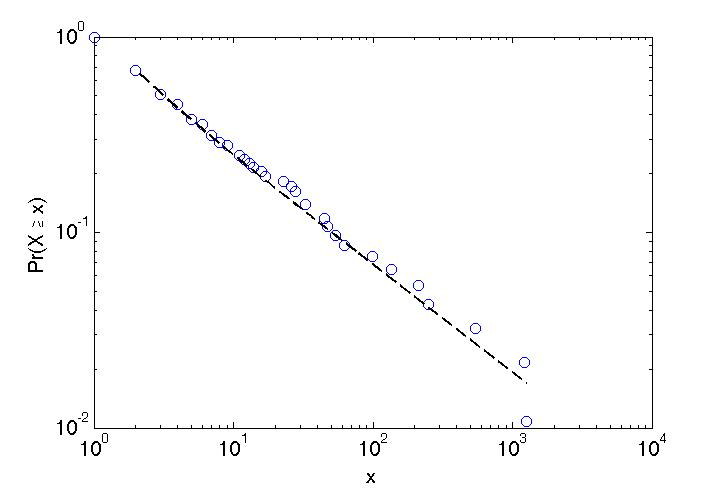
\includegraphics[scale=0.35]{3.Chapter1/Media/retweets-distribution-stats.jpg} 
\caption{\textit{Maximum likelihood power-law fit for the cumulative distribution of retweet group sizes.}}
\label{fig:retweet-distribution}
\end{figure}
\begin{figure}[h]
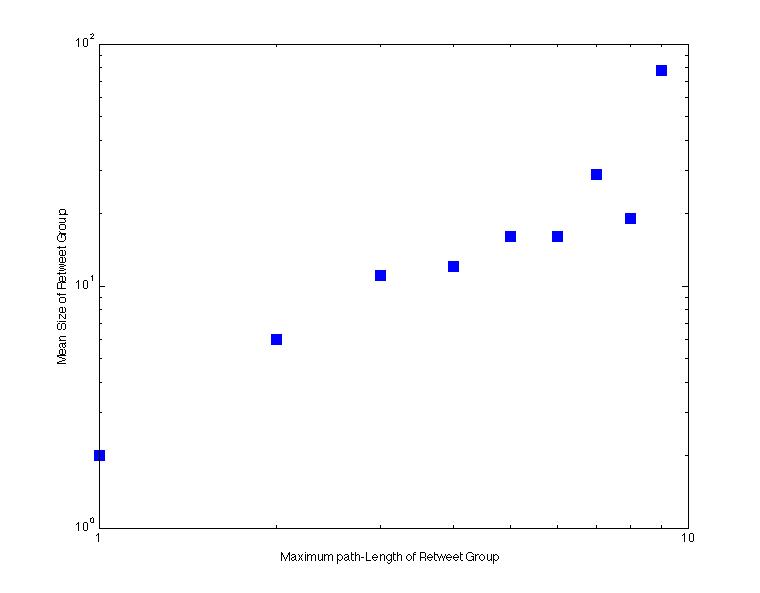
\includegraphics[scale=0.35]{3.Chapter1/Media/retweets-pathlength.jpg} 
\caption{\textit{Log/log relationship between the maximum path-length and size of a retweet group.}}
\label{fig:totalretweets-pathlength}
\end{figure}
Figure \ref{fig:totalretweets-pathlength} shows how the total number of retweets varies with the longest path-length of the retweet group. The trend mostly correlates with what might be expected; that the maximum path-length of a group increases with the overall size of the group. These illustrations do not show which users are followers of others, but do show how some tweets are retweeted significantly more than others. Users who have many more followers are said to be more \textit{influential}, say Cha M. et al. \cite{cha10}, who also discuss the idea of `indegree', and that those users who have far more followers than friends are likely to be far more influential. Their chance of having tweets retweeted is therefore increased.\\
The (immediate) audience size of a retweet group refers to the number of users the tweet has been exposed to either directly or through retweets. \textit{Immediate} was used in this sense since users who have made their profile public can have their tweets viewed by users who aren't followers of the former. This audience size can therefore be calculated simply by summing up all the followers of each of the users in the retweet group.\\
\begin{figure}[h]
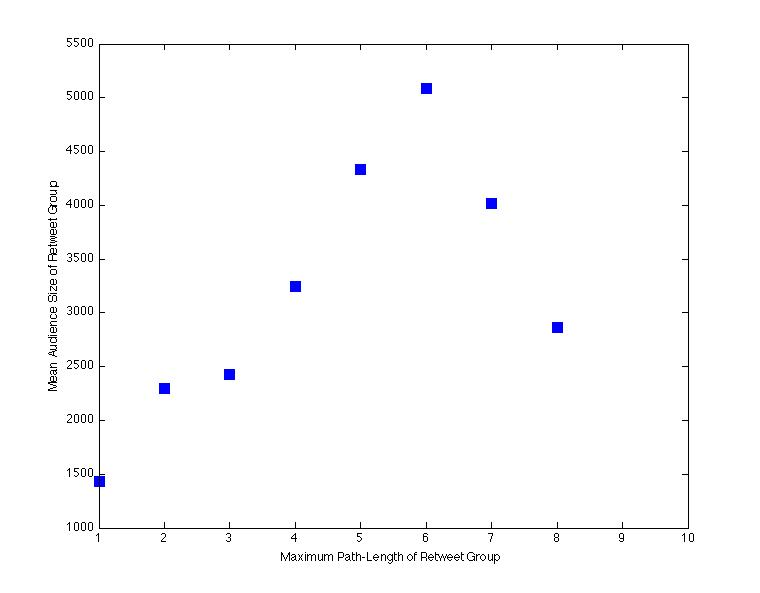
\includegraphics[scale=0.35]{3.Chapter1/Media/audience-pathlength.jpg} 
\caption{\textit{Relationship between a retweet group's audience size and its longest path-length.}}
\label{fig:pathlength-audience}
\end{figure}
These audience measures take into account that some users may be exposed to the same tweet more than once. This happens when users involved in a retweet tree have some followers in common, and so is likely to be prevalent in more closely-knit communities. As a result, the audience sizes shown only represent \textit{distinct} users exposed to the tweet.\\
Collection of the audience size from the data started slightly later than the main dataset and is only available for 2860 of the total 4400 groups. The longest maximum path-length of this subset is 8.\\
Figure \ref{fig:pathlength-audience} shows how the audience size of retweet groups varies with their maximum path-length. The peak at path-length 5 indicates that the groups with a mid-range maximum path-length tend to have a larger audience size, and we believe this is to do with the amount of audience overlap in different retweet groups.\\
\cite{kwak10} discusses how retweeting is related to the audience size of a tweet and how the power of the retweet phenomenon can greatly affect the spread of information, even if the original tweeter has only a few followers. The same paper more specifically mentions that the audience size of a retweeted tweet reaches, on average, at least 1,000 users, no matter the number of followers of the original tweeter. This can also be seen in our results; that no matter the maximum path-length of a tweet, the number of users reached is relatively high.\\
The overhead of a retweet group represents the number of users who are exposed to a tweet more than once and is present in 71\% of retweet groups. The \textit{proportionate} overhead is the ratio of overhead to audience size and the mean of this was found to increase with the group's maximum path-length. This is a possible explanation for the peak in the data: that eventually the overhead of non-distinct users has increased to the extent that it reduces the audience size more significantly. The same graph representing the effective audience size (calculated with the addition of non-distinct users) represents, mostly, a continuous positive correlation.\\
Three of the largest five overheads collected were from retweet groups with a maximum path-length of 1, the largest with an overhead of 6.5 times greater than the distinct audience itself (the overhead was larger than the actual audience size in around 3\% of retweet groups). This shows that, to an extent, there can be significantly more overlap in more closely-knit communities; those retweet trees which are wide and shallow. The chance of getting no overhead increases in smaller retweet groups.

\subsection{Retweet Follower Pattern}
\label{retweet follower pattern}
This experiment focuses on the pattern of followers in the retweeting hierarchy.\\
The first result shown from the experiment is that the final retweeter follows the previous retweeter in the chain in 67\% of cases. It initially seems strange that this should be 20\% lower than when following a user in retweet chains of length one. This suggests that users involved in shorter-chain path-length retweets are members of more tightly-knit communities. Retweets with longer path-lengths have, by nature, travelled further and so would be the type of retweet to travel between communities, reducing the chance of the involved users following each other.\\
The interesting part of this, however, is the number of followers of the previous retweeter in different cases. In the 33\% of cases where the final retweeter doesn't follow the previous retweeter, the latter has, on average, around 600 followers. When the final retweeter \textit{does} follow the previous retweeter, however, the previous retweeter's average number of followers is 940. This is quite a substantial difference and certainly highlights the fact that by having more followers you are more likely to have more influence in terms of whether you get retweeted, or not.\\
This is accentuated further when looking at the original tweeter. The likelihood of a retweeter following the original tweeter in cases in which the path-length is of more than one has already been found to be around 40\%, but the average number of followers of the original tweeter increases by a factor of around four (580 to 2000) when also followed by the final retweeter. Results showed that the original tweeter had a consistently higher number of followers when followed by the final retweeter than when not at all path-lengths. This demonstrates that having an increased number of followers is correlated with the chance of a user being retweeted. In this case, having four times the followers increases the correlation dramatically (40\% to 90\%). The number of followers of a user can therefore be directly related to the ideas of influence discussed in \cite{cha10} and also of `advertising' themselves.\\
\begin{figure}[h]
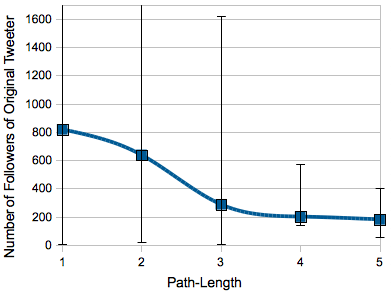
\includegraphics[scale=0.6]{3.Chapter1/Media/originalfollowers-pathlength-distribution.png} 
\caption{\textit{Relationship between number of followers (and respective distribution) of the original tweeter as the path-length increases.}}
\label{fig:originalfollowers-pathlength}
\end{figure}
It was found, however, that the number of followers of the original tweeter diminishes as the path-length of the tweet increases (Figure \ref{fig:originalfollowers-pathlength}), signifying that tweets travel further when the original tweeter has fewer followers. Because the retweet groups were collected in such a way so that groups containing longer path-length retweets also contained many shorter-chain retweets, retweet groups containing path-lengths of 5 (or more) are also likely to contain many retweets (if not more) with path-lengths of one or two (see the distribution in Figure \ref{fig:pathlength-distribution}). It can therefore be argued that there are more users involved in shorter-chain retweets than in ones with longer path-lengths. It is then more likely for these users to have more followers than others in the retweet group. Another explanation could be that users are actually aware of their local network and realise that retweeting may cause a lot of audience overlap (particularly in the case of large communities). A user may have seen a post retweeted a few times on their home timeline and thus decide not to also retweet.\\
One last interesting point to make regarding the notion of retweet chains is looking at the how the pattern of following previous retweeters develops as the path-length increases. It has already been discussed above how the chance of following the previous retweeter in the chain is about 67\%, but, in cases where the path-length of a tweet is greater than two (i.e. at least two intermediate retweeters between final retweeter and original tweeter), the chance of the final retweeter following the next retweeter along preceding the previous retweeter is around 45\%. This suggests that retweeting is more widespread and not so much just circulated around communities. These preliminary results demonstrate that the chance of the final retweeter following previous retweeters - up to and including the original tweeter - diminishes along the chain or as the tree is ascended (Figure \ref{fig:following-possibility}).\\
\begin{figure}[h]
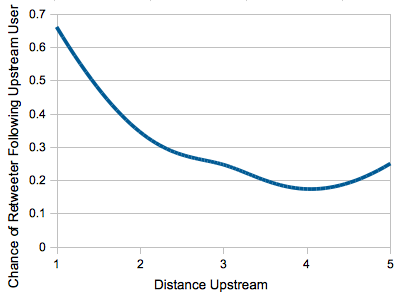
\includegraphics[scale=0.55]{3.Chapter1/Media/following-possibility.png} 
\caption{\textit{Proportion of final retweeters following upstream users at varying distances along the chain.}}
\label{fig:following-possibility}
\end{figure}
Because of this, it's sensible to assume that the tweets in the dataset are forwarded through less-connected users, and perhaps forwarded from community to community by those users belonging to several groups. Otherwise, if the retweets were circulated more around closely-knit communities, the likelihood of the final retweeter following the previous tweeters would be both greater and more evenly spread - i.e. the chance of following the previous retweeter would be roughly equal to the chance of following the other tweeters in the chain.\\
In addition, of the 67\% of final retweeters who \textit{are} following the previous retweeter, about 19\% of them also follow the next previous retweeter (i.e. the retweeter at path-length - 2). In this case, the next previous retweeter has, on average, 3000 followers. In the 81\% of these users \textit{not} following the next previous retweeter, then the latter has an average of 525 followers. This is an accentuated result of the one previously, but this time boasts an increase of a factor of 6.\\
Of the 33\% of users who \textit{don't} follow the previous retweeter, about 30\% follow the next previous retweeter. Both of these sets of statistics also go towards the idea of the diminishing chance of following the users as the tree is ascended.\\
From this dataset, it was also possible to work out how often retweeters cited the original tweeter of a post. In retweets, users are typically cited by, as we have seen, having their name along with an `RT' at the start of the post. This data was collected by seeing if the original poster's username was mentioned \textit{anywhere} in each retweet. The chance of this occurring was found to be around 68\% and did not vary with any pattern with path-length.
 
\subsection{Retweet Time Delay}
\label{retweet time delay}
The final experiments in this section focus on the time delay between the final retweeter and original tweeter. This is an interesting area since it enables researchers to see how fast messages propagate through the Twittersphere. From this information, and by using the retweeter patterns demonstrated above, it would be possible to work out how far and how quickly information can be passed around.\\
Figure \ref{fig:timedelay-pathlength} shows the average time delay between the first and final retweet with increasing maximum path-length of the retweet group.\\
\begin{figure}[h]
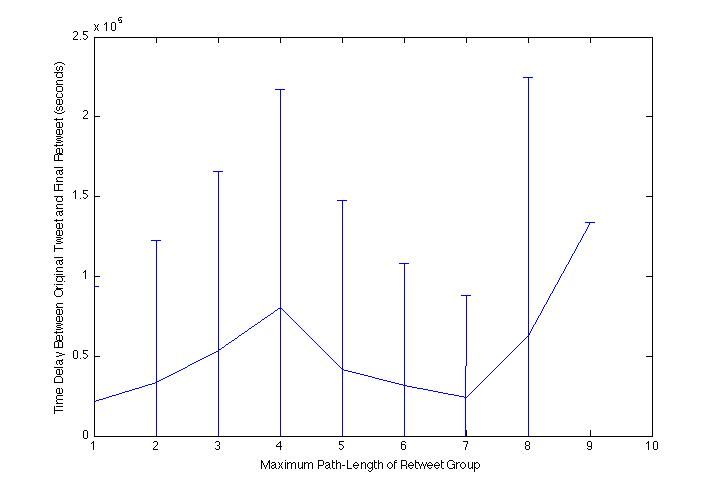
\includegraphics[scale=0.35]{3.Chapter1/Media/pathlength-timedelay.jpg} 
\caption{\textit{Average time (in seconds) between first post and final retweet of a retweet group varying with the group's maximum path-length.}}
\label{fig:timedelay-pathlength}
\end{figure}
The results indicate that, mostly, as the group's maximum path-length increases, then so does the elapsed time between the original post and the final retweet. This is probably as was expected, since this shows that it takes longer for a retweet to travel further. The data is not consistent, however, especially results for a path-length of five and above. The first four results suggest a uniform incline roughly proportional to $ v=\frac{s}{t} $, where the distance, \textit{s}, is the hypothetical distance given by the path-lengths, showing that the \textit{speed} of propagation remains mostly constant.\\
There is not enough of a trend in the data to make any deductions regarding propagation speed, however. There are two main conflicting arguments regarding this result: the first is, as mentioned, that the further a tweet travels the longer time it travels for. The second is to do with tweet popularity: the more popular a tweet is, the more quickly it will be retweeted. In the latter case, it is possible that longer trees grow fully before shorter ones, implying exponential growth. Generally, though, it seems that the maximum path-length of a retweet group does not massively affect the tweet's propagation speed.

\section{Summary}
\label{analysis}
The experimental results have certainly highlighted the ideas of communities and that of message cascading similar to that demonstrated in \cite{java07} and \cite{galuba10} respectively.\\
As has been seen, in section \ref{retweet time delay}, the retweet tree seems to grow in a variety of ways. One argument is mostly expected; that as the `distance' the tweet travels increases, then so does the time taken for it to reach its end. The other argument is linked to the idea of tweet advertising, discussed in previous sections, and namely the notion of tweet popularity.\\
The previous experiments showed how the number of followers of a user directly influences their chance of being retweeted. It can therefore be seen that advertising can also be linked to the level of influence a user has. The results help illustrate the multi-dimensional properties of the retweet tree, and how these factors relate to its growth and its associated friend-follower graph.

%\section{Conclusions}
This paper has demonstrated relatively simple results in an attempt to realise some of the behavioural patterns of retweets, both linking to the psychologically in terms of the users, but also the physical properties of retweets. The results are able to represent a basis for potential further work and research into the various aspects of Twitter, moreover, perhaps, topical categorisation and the dynamicity of the friend-follower graphs.
